\chapter{Umsetzung der Use-Cases und Evaluation} \label{Umsetzung der Use-Cases und Evaluation}

\section{Use-Case 1: Basis Deployment} \label{Use-Case 1: Basis Deployment}
%IPAM-Vorbereitungen, TF Matching erläutern
%Was ist ein Subnet im Cloud-Kontext? Einleitung?
%TF: Resource, Data, Modul, Provider
\subsection{Umsetzung: Kerntätigkeiten}

Im phpIPAM müssen mehrere Netzbereiche reserviert werden. Es werden Netzbereiche benötigt, in denen Maschinen per IPv4 kommunizieren können. Diese Netze werden mit VPC bzw. VNET assoziiert.\\
Für VNET wurde der Netzblock \glqq 10.32.0.0/16\grqq{} und für VPC der Netzblock \glqq 10.33.0.0/16\grqq{} vorreserviert, aus dem kleinere Subnets für die jeweilige Cloud entnommen werden können. Weiterhin ist die Annahme, dass die Private Cloud bereits einen Netzbereich besitzt, in dem Maschinen angesiedelt sind: \glqq 192.168.201.0/24.\grqq{}\\
Es werden {Transfernetzwerke} benötigt, über die die IPv4-Pakete geschickt werden und die BGP-Präfixe ausgetauscht werden können. AWS sieht hierfür /30-Präfixe aus dem Bereich \glqq 169.254.0.0/16\grqq{} vor \cite{awsvpn2021}, Azure hat eine Range reserviert: \glqq 169.254.21.0\grqq{} -\\ \glqq 169.254.22.255\grqq{} \cite{azurebgp2020}. Als Kompromiss können daher nur Netze aus den Azure-Bereichen genutzt werden, da die Bereiche, die AWS zur Verfügung stellt, größtenteils außerhalb dieser Range liegen. Auch diese Netzbereiche müssen im IPAM vorreserviert werden und für die Transfernetzwerke automatisiert konfiguriert werden.\\
In Beispiel \ref{apipa-reservation-ipam} wird in phpIPAM nach dem Bereich \glqq TF\_CLOUD\_BGP\_TRANSFER\grqq{}, aus dem alle Transfernetzwerke entommen werden, gesucht. Innerhalb des Bereichs wird aus dem vorreservierten Block \glqq Cloud\_Transfer\_BGP\_1\grqq{} ein /30-Netzwerk entnommen. Die Reservierung der Netzblöcke für VPC und VNET erfolgen analog.
%TC:ignore
\begin{listing}[h]
\begin{minted}[breaklines,frame=single]{tf}
//Azure - AWS Transfer
data "phpipam_section" "apipa_main_section" {
  name = "TF_CLOUD_BGP_TRANSFER"
}
data "phpipam_subnet" "apipa_transfer_subnet" {
  section_id = data.phpipam_section.apipa_main_section.section_id
  description_match = "Cloud_Transfer_BGP_1"
} 
resource "phpipam_first_free_subnet" "free_subnet_apipa" {
  parent_subnet_id = data.phpipam_subnet.apipa_transfer_subnet.subnet_id
  subnet_mask = 30
  description = "BGP_AWS_AZURE"
}
\end{minted}
\caption{Die data-Anweisungen dienen ausschließlich der Suche nach dem passenden Transfernetzwerk-Block. Per resource-Anweisung wird ein /30-Netzwerk reserviert.}
\label{apipa-reservation-ipam}
\end{listing}\FloatBarrier
%TC:endignore
Weiterhin werden Pre-Shared-Keys für die Aushandlung der IPsec-Verbindungen benötigt. AWS erzeugt automatisch solche Schlüssel, welche durch die Terraform-Resource \glqq aws\_vpn\_connection\grqq{} zurückgegeben werden. Diese automatisch erzeugten Schlüssel werden daher für die Backbone-Verbindungen AWS $\leftrightarrow$ Azure und AWS $\leftrightarrow$ Private Cloud genutzt. Da Azure diese Schlüssel nicht erzeugt, wurde ein Terraform-Modul geschrieben, welches 24 Zeichen lange Schlüssel erzeugt. Diese können anschließend genutzt werden für die Backbone-Verbindung Azure $\leftrightarrow$ Private Cloud.
%TC:ignore
\begin{listing}[h]
\begin{minted}[breaklines,frame=single]{tf}
resource "random_password" "random_password" {
  length = 24
  lower = true
  upper = true
  number = true
  special = false
}
output "azure_vyos_tunnel1_psk" {
  value = random_password.random_password.result
  sensitive = true
}
\end{minted}
\caption{Auf Sonderzeichen (special) wurde verzichtet. Das Modul stellt per output-Anweisung den Schlüssel für andere Terraform-Module zur Verfügung.}
\label{tf-generate-psk}
\end{listing}\FloatBarrier
%TC:endignore
%alles Devices nennen?
Da, wie bereits erwähnt, für die VyOS-Router keine \textit{native} Terraform-Integration verfügbar ist, wurde zur Konfiguration des Devices eine Vorlage erstellt, welchi per CLI Konfigurationen ausrollt.

%https://www.terraform.io/docs/language/functions/templatefile.html
Die Erzeugung der Vorlage erfolgt über die Funktion templatefile() \cite{templatefiletf2021}.

%TC:ignore
\begin{listing}[h]
\begin{minted}[breaklines,frame=single]{tf}
resource "local_file" "vyos_config" {
  filename = /tmp/example.sh
  content = templatefile("${path.module}/include/vyos_config.tpl",
  {
    aws_vgw_ip = var.aws_vgw_ip
    aws_tunnel1_psk = var.aws_tunnel1_psk
  })
}

\end{minted}
\caption{Die Funktion templatefile() erzeugt aus einer Template-Datei \underline{vyos\_config.tpl} die Datei \underline{/tmp/example.sh}. Die Template-Datei wird mit den Variablen \textit{var.aws\_vgw\_ip} und \textit{aws\_tunnel1\_psk} befüllt.}
\label{tf-call-tpl-generation}
\end{listing}\FloatBarrier
%TC:endignore
%TC:ignore
\begin{listing}[h]
\begin{minted}[breaklines,frame=single]{bash}
$ head -n 11 < vyos/include/vyos_config.tpl
#!/bin/vbash
source /opt/vyatta/etc/functions/script-template
configure
#AWS
set vpn ipsec ike-group AWS lifetime '28800'
set vpn ipsec ike-group AWS proposal 1 dh-group '2'
set vpn ipsec ike-group AWS proposal 1 encryption 'aes128'
set vpn ipsec ike-group AWS proposal 1 hash 'sha1'
set vpn ipsec site-to-site peer ${aws_vgw_ip} authentication mode 'pre-shared-secret'
set vpn ipsec site-to-site peer ${aws_vgw_ip} authentication pre-shared-secret ${aws_tunnel1_psk}
set vpn ipsec site-to-site peer ${aws_vgw_ip} description 'VPC tunnel 1'

\end{minted}
\caption{Verschiede set-Kommandos werden in ein VyOS-Skript eingebettet (Interpreter: \texttt{/bin/vbash}). Die Variablen in Zeilen 9-12 resultieren aus dem Funktionsaufruf (s. Beispiel \ref{tf-call-tpl-generation}).}
\label{tf-generate-tpl}
\end{listing}\FloatBarrier
%TC:endignore
%TC:ignore
\begin{listing}[h]
\begin{minted}[breaklines,frame=single]{tf}
resource "null_resource" "vyos_config" {
  connection {
    type = "ssh"
    host = var.vyos_host
    user = var.ssh_user
    private_key = file(var.private_key_file)
  }
  provisioner "file" {
   source = /tmp/example.sh
   destination = var.vyos_script_path
  }
  provisioner "remote-exec" {
    inline = [ "chmod +x ${var.vyos_script_path}", var.vyos_script_path ]
  }
}
\end{minted}
\caption{Das in \ref{tf-generate-tpl} generierte Shell-Skript wird per \texttt{ssh} auf das Zielsystem (VyOS-Router) kopiert und per Provisioner \textit{remote-exec} ausgeführt.}
\label{tf-copy-tpl}
\end{listing}\FloatBarrier
%TC:endignore
Folgend werden Probleme erläutert, die bei dieser technischen Umsetzung auftraten und wie eine Lösung erarbeitet wurde.
\newpage
\subsection{Probleme und Lösungsfindung}
%Probleme: Race Condition externe IP, Redeploy wegen TF Bug, statische Route zu BGP Neighbor (Azure - AWS: Pseudo directly, Azure - VyOS: Static, Azure - AWS), stateless VyOS Config, lange Laufzeiten Erstellung VPN Gateway Azure

\textbf{\underline{Vertauschung von IPsec-Tunnelparametern}}\label{xml-tunnel-parameters}

AWS VPN-Konzentratoren bieten aus Redundanzgründen standardmäßig zwei IPs pro Gegenstelle an. 
%TC:ignore
\begin{listing}[h]
\begin{minted}[breaklines,frame=single]{xml}
<?xml version="1.0" encoding="UTF-8"?>
<vpn_connection id="vpn-096f7fc91dc77cc74">
  [...]
  <ipsec_tunnel>
    <vpn_gateway>
      <tunnel_outside_address>
        <ip_address>18.194.163.131</ip_address>
      </tunnel_outside_address>
      [...]
    </vpn_gateway>
    <ike>
      [...]
      <pre_shared_key>B28VDw7xcqYJZvcWCI7E</pre_shared_key>
    </ike>
    [...]
  </ipsec_tunnel>
  <ipsec_tunnel>
    [...]
    <vpn_gateway>
      <tunnel_outside_address>
        <ip_address>35.157.252.106</ip_address>
      </tunnel_outside_address>
    [...]
    </vpn_gateway>
    <ike>
      [...]
      <pre_shared_key>cHgnL5wZ1vPGTdHhbuLW</pre_shared_key>
    </ike>
    [...]
  </ipsec_tunnel>
</vpn_connection>

\end{minted}
\caption{Die ursprüngliche (gekürzte) XML-Antwort der AWS API.}
\label{tf-xml-response-aws}
\end{listing}
%TC:endignore
Wie man sieht, taucht das XML-Element ipsec\_tunnel zwei Mal auf, ist dabei jedoch \textbf{unnummeriert}.
Der Terraform-Provider aws\_vpn\_connection nutzt diese XML-Antwort, um daraus die Rückgabewerte tunnel1\_* und tunnel2\_* zu erzeugen\cite{awsattributestf2021}, die in der weiteren Ausführung von anderen Modulen wiederverwendet werden. Bei einigen Ausführungen wurden diese Elemente Terraform-intern vertauscht: Da nun weder IPsec-Schlüssel noch interne BGP-Peering-Gegenstellen stimmen, kommen weder IPsec-Tunnel noch die BGP-Peering-Sessions hoch. Dieser Bug ist in Github für den AWS Provider seit 2017 dokumentiert\cite{githubbugtf2021}.

Mit einem Bash-Skript konnte zumindest ein Workaround gefunden werden, um ein erfolgreiches Deployment sicherzustellen. Die Grundannahme ist, dass pro Präfix zwei Pfade auf dem Private Cloud-Router existieren. Wenn nur ein Pfad pro Präfix zur Verfügung steht, kam es mit einer hohen Wahrscheinlichkeit zu einer Vertauschung und es wird redeployed (\texttt{terraform destroy \&\& terraform apply}). Es wird dreimal versucht, eine funktionierende Infrastruktur zu deployen, um die APIs der Cloud-Anbieter zu \textit{schonen} und kein Rate-Limiting zu triggern \cite{awsthrottling2021}.
%TC:ignore
\begin{listing}[h]
\begin{minted}[breaklines,frame=single]{bash}
vyos@vyos-cloud:~$ sh ip bgp | grep -A1 -E '10.3[2|3]'
*  10.32.0.0/16     169.254.53.1    100     0   65516 65515 i
*>                  169.254.21.6            0   65515 i
*  10.33.0.0/24     169.254.21.6            0   65515 65516 i
*>                  169.254.53.1    100     0   65516 i

\end{minted}
\caption{BGP-Präfixe und dazugehörige AS-Pfade (rechts) auf dem VyOS-Router. Beide Präfixe sind redundant über zwei Pfade zu sehen (Deployment erfolgreich).}
\label{bgp-paths-vyos}
\end{listing}
%TC:endignore
\newpage
Beispiel \ref{grafik:programmablaufplan_bash_deploy_tf} zeigt den Programmlaufplan des Bash-Skripts \texttt{deploy.sh}. Wenn weniger als zwei Pfade pro Präfix gesehen, findet ein \textit{Re-Deployment} statt.

\begin{figure}[h]
  \centering
  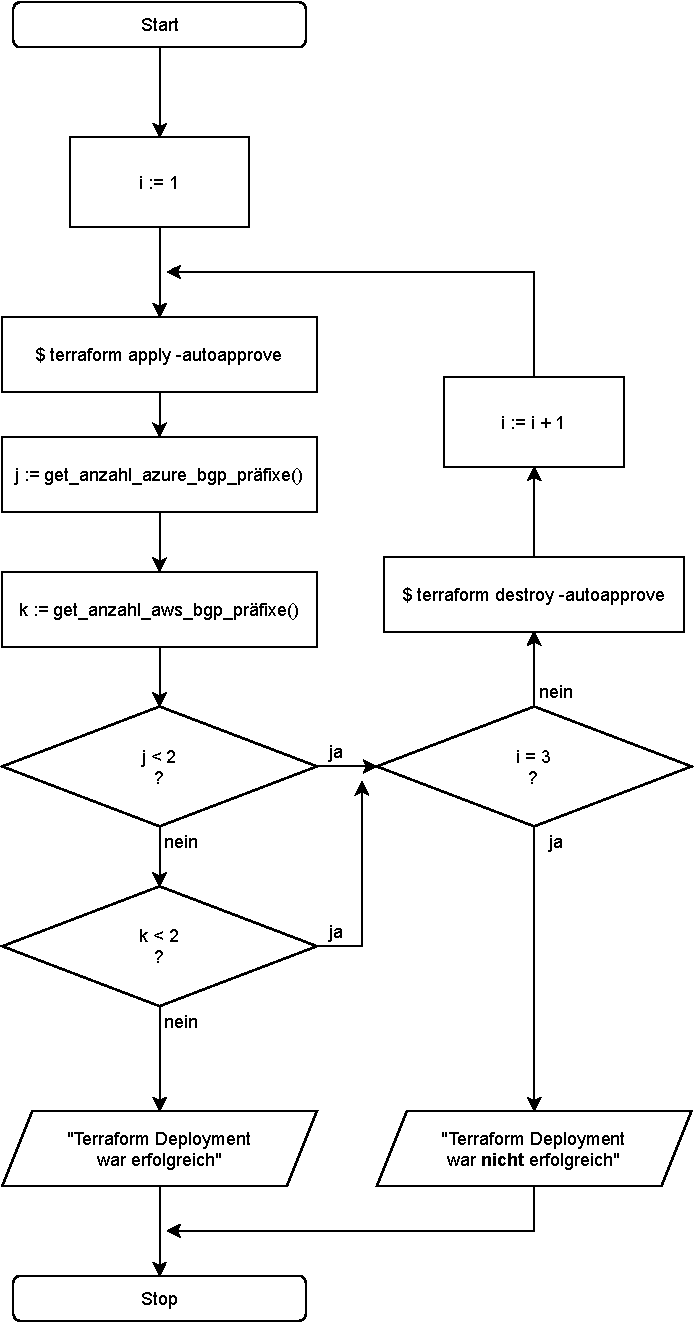
\includegraphics[scale=0.6]{Figures/programmablaufplan_bash_deploy_tf.pdf}
  \caption{Programmablaufplan für das Terraform Deployment Skript}
  \label{grafik:programmablaufplan_bash_deploy_tf}
\end{figure}\FloatBarrier

Durch das Bash-Skript wurde dieser Bug nicht zum \textit{Showstopper}, allerdings führten Redeployments zu relativ langen Deployment-Zeiten (siehe auch \ref{azure-deployment-time}).

Anmerkung: Dieser Bug wurde angeblich noch kurz vor Abgabe dieser Arbeit behoben. Das konnte allerdings nicht mehr verifiziert werden. Es ist im Commit ersichtlich, dass es sich um einen Bug in der internen Sortierfunktion handelt.\cite{awsfixtf2021}

\textbf{\underline{Zustandslose VyOS-Konfiguration}}\\
%Terraform Einleitung
Terraform speichert, wie bereits erläutert, alle Referenzen auf Infrastrukturkomponenten in der Datei terraform.tfstate. Da es für VyOS keinen vollwertigen Terraform-Provider gibt, wurde mit Templates, die verschiedene \texttt{set}-Kommandos ausführen, gearbeitet.\\
Diese Konfigurationsänderungen sind dadurch völlig zustandlos, da sie nicht invertierbar sind: Terraform kennt nicht die Umkehrung der \texttt{set}-Kommandos, welche benötigt würden, um bei einen \texttt{terraform destroy} die Konfigurationen am VyOS-Router rückgängig zu machen.

Ein Ansatz wäre gewesen, ein weiteres Template zur Verfügung zu stellen, in dem alle \texttt{set}- durch \texttt{delete}-Kommandos negiert werden.\\
%TC:ignore
\begin{listing}[h]
\begin{minted}[breaklines,frame=single]{bash}
vyos@vyos-cloud# set system time-zone Europe/Berlin
[edit]
vyos@vyos-cloud# delete system time-zone Europe/Berlin
[edit]
\end{minted}
\caption{VyOS: \texttt{delete} negiert das vorherige \texttt{set}-Kommando.}
\label{set-delete-vyos}
\end{listing}
%TC:endignore
Per \textit{Destroy-Time Provisioner} würde dieses Template nur bei einem \textit{terraform destroy} genutzt\cite{destroytimeprovtf2021}. Das Problem ist, dass schon bei minimalen Änderungen des Deploy-Templates auch das Destroy-Template angepasst werden muss.
Außerdem sind die IPsec-Konfigurationen relativ umfangreich. Es war zu anzunehmen, dass Relikte aus der Konfiguration übrig bleiben, wenn die Negation aus unbekannten Gründen fehlschlug.
Eine weitere Idee war, mit dem VyOS-Feature \textit{rollback} zu arbeiten. Über eine commit-History werden alle Änderungen an dem System dokumentiert.
%TC:ignore
\begin{listing}[h]
\begin{minted}[breaklines,frame=single]{bash}
vyos@vyos-cloud:~$ show system commit | head -3
0   2021-05-05 09:47:51 by tf via cli
1   2021-05-05 09:25:24 by tf via other
2   2021-05-04 21:17:57 by vyos via cli

\end{minted}
\caption{VyOS: Die commit history speichert alle gemachten Änderungen und macht sie revisionssicher.}
\label{commit-history-vyos}
\end{listing}\FloatBarrier
%TC:endignore
So würde man die letzte Revision \textit{vor} der Konfiguration der Backbone-Verbindungen festhalten, um bei einem \texttt{terraform destroy} darauf zurückgehen zu können.
%TC:ignore
\begin{listing}[h]
\begin{minted}[breaklines,frame=single]{bash}
vyos@vyos-cloud# rollback
Possible completions:
  <N>   Rollback to revision N (currently requires reboot)

  Revisions:
    0   2021-05-05 09:47:51 tf by cli
    1   2021-05-05 09:25:24 tf by other
    2   2021-05-04 21:17:57 vyos by cli
    
\end{minted}
\caption{VyOS: Rollback auf Revision $N$ nach Reboot}
\label{rollback-cmd-vyos}
\end{listing}\FloatBarrier
%TC:endignore
Es wurden zwei Bash-Skripte geschrieben: \texttt{save\_last\_manual\_commit.sh} speichert die letzte Revision lokal auf dem VyOS-Router, \texttt{apply\_last\_manual\_commit.sh} macht ein Rollback.
%TC:ignore
\begin{listing}[h]
\begin{minted}[breaklines,frame=single]{tf}
resource "null_resource" "vyos_config" {
  connection {
    type = "ssh"
    host = var.vyos_host
    user = var.ssh_user
    private_key = file(var.private_key_file)
  }
  [...]
  provisioner "local-exec" {
    command = "${path.module}/bin/save_last_manual_commit.sh"
  }
}

\end{minted}
\caption{Terraform kopiert per \texttt{ssh} ein Skript auf den VyOS-Router, welches den Zustand vor Deployment \glqq einfriert\grqq{}.}
\label{save-last-commit-vyos}
\end{listing}\FloatBarrier
%TC:endignore
Nach \textit{terraform apply} liegt auf dem VyOS-Router eine Datei, die den letzten Timestamp der speichert.
%TC:ignore
\begin{listing}[h]
\begin{minted}[breaklines,frame=single]{bash}
vyos@vyos-cloud# cat ~tf/last_manual_commit.txt
2021-05-05 09:47:51 by tf via cli
\end{minted}
\caption{Timestamp des letzten (manuellen) commits vor Deployment per Terraform.}
\label{save-last-commit-file}
\end{listing}\FloatBarrier
%TC:endignore
Bei \texttt{terraform destroy} wird das Skript \texttt{apply\_last\_manual\_commit.sh} via Terraform \texttt{Destroy-Time Provisioner} ausgeführt, welches den Rollback hin zu dem gespeicherten Zeitpunkt auf dem VyOS Router veranlasst.
%TC:ignore
\begin{listing}[h]
\begin{minted}[breaklines,frame=single]{tf}
resource "null_resource" "vyos_config_destroy" {
  provisioner "local-exec" {
    when = destroy
    command = "${path.module}/bin/apply_last_manual_commit.sh"
  }
}

\end{minted}
\caption{Bei \texttt{terraform destroy} wird ein Skript auf den VyOS-Router kopiert, welches die Änderungen mit Hilfe des Timestamps aus \ref{save-last-commit-file} rückgängig macht.}
\label{apply-last-commit-vyos}
\end{listing}\FloatBarrier
%TC:endignore
\textbf{\underline{Lange Laufzeiten für Erstellung von Azure VPN Gateway}}\label{azure-deployment-time}\\
Die Erstellung des Azure VPN Gateways kann bis zu 45 Minuten in Anspruch nehmen \cite{azurevpndeployment2021}. In der Praxis waren es meist etwa 25 Minuten für den Standort \glqq North Europe\grqq{}. Auch das Löschen eines VPN Gateways via \texttt{terraform destroy} dauert bis zu 15 Minuten. Nur wenn dieses Gateway gelöscht wurde, kann ein \textit{Re-Deployment} erfolgen, welches vor allem dann notwendig ist, wenn die Vertauschung von IPsec-Parametern (siehe \ref{xml-tunnel-parameters}) eintrifft.\\
Bei diesem Phänomen handelt es sich nicht um einen Bug im eigentlichen Sinne, macht aber das Deployment z.B. für Live-Demonstrationen nicht praktikabel. Da alle weiteren Use-Cases auf diesem Use-Case 1 aufbauen und ebenso in Terraform abgebildet werden sollten, musste eine Lösung gefunden werden, um die Deployment-Zeiten zu verkürzen, da jede Änderung des Codes ein (teilweises) Re-Deployment notwendig macht (vgl. später).

%Dies wird zum Beispiel gebraucht, wenn an der Konfiguration der Infrastruktur Änderungen vorgenommen werden, da Terraform durch diese State-Datei weiß, dass 
%TC:ignore
\subsection{Evaluation}
Nach dem erfolgreichen Deployment wird folgender Status von Terraform zurückgemeldet:
\begin{listing}[h]
\begin{minted}[breaklines,frame=single]{bash}
Apply complete! Resources: 29 added, 0 changed, 0 destroyed.

Outputs:

aws_subnet_id = "subnet-0192ae38a3a16f584"
[... weitere Output-Variablen ...]
\end{minted}
\caption{Terraform Status nach Deployment Use-Case 1}
\label{tf-base-deployment-ok}
\end{listing}
%TC:endignore
Die im IPAM reservierten Netze sind in AWS als Subnets wiederzufinden. Die Prüfung analog für Azure ist ebenso erfolgreich.

\begin{figure}[h]
  \centering
  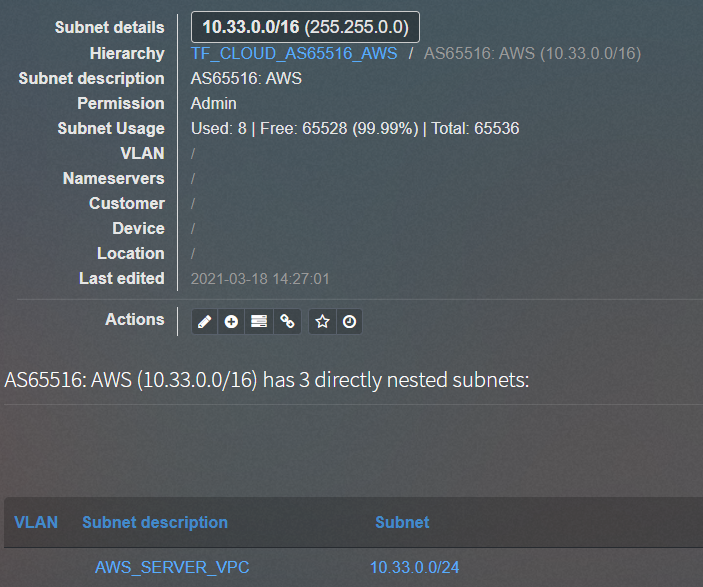
\includegraphics[scale=0.8]{Figures/subnet_aws_ipam_server.png}
  \caption{Es wurde ein Subnet für AWS (Server) reserviert.}
  \label{grafik:subnet_aws_vpc_ipam_reserved}
\end{figure}

\begin{figure}[h]
  \centering
  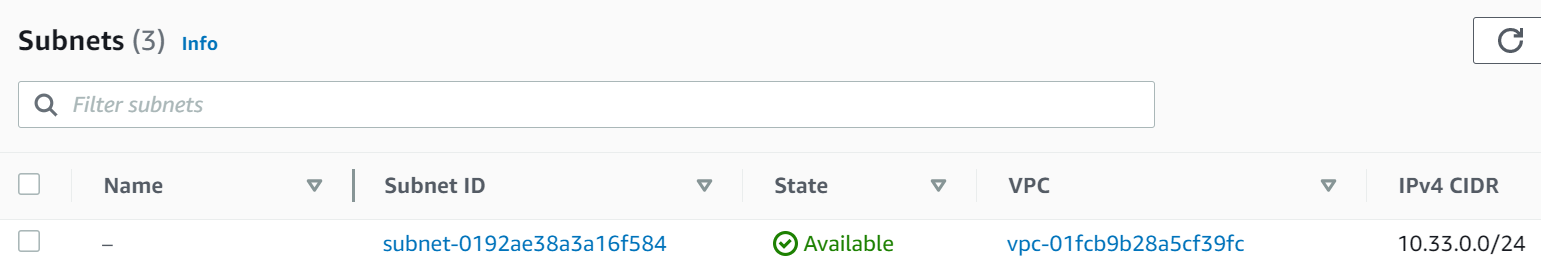
\includegraphics[scale=0.4]{Figures/subnet_aws_reserved_server.png}
  \caption{Das Subnet findet sich in AWS wieder.}
  \label{grafik:subnet_aws_vpc_reserved}
\end{figure}\FloatBarrier

Die IPsec Tunnel sind auf dem VyOS-Router konfiguriert und \textit{up}.
%TC:ignore
\begin{listing}[h]
\begin{minted}[breaklines,frame=single]{bash}
vyos@vyos-cloud:~$ show vpn ipsec sa
Connection                     State    Uptime
-----------------------------  -------  --------
[...]
peer-20.67.209.254-tunnel-vti  up       4h43m19s [...]
peer-3.65.181.187-tunnel-vti   up       4h47m26s [...]

\end{minted}
\caption{VyOS: IPsec Status}
\label{tf-base-deployment-ipsec-ok}
\end{listing}\FloatBarrier
%TC:endignore
Die Adressen gehören dabei zu Amazon bzw. Microsoft.
%TC:ignore
\begin{listing}[h]
\begin{minted}[breaklines,frame=single]{bash}
$ whois 3.65.181.187 | grep -A2 NetRange
NetRange:       3.64.0.0 - 3.79.255.255
CIDR:           3.64.0.0/12
NetName:        AMAZON-FRA

\end{minted}
\caption{Diese Adresse gehört Amazon. Analog wurde geprüft für 20.67.209.254 (Microsoft).}
\label{whois-amazon-public-ip}
\end{listing}
%TC:endignore
Außerdem wurden auf dem Cloud-Router die AWS- und Azure-Präfixe via BGP installiert. Pro Präfix sind zwei Pfade vorhanden (s. Beispiel \ref{bgp-paths-vyos}).

Es wurde pro Cloud eine virtuelle Maschine (Ubuntu) installiert, um die Ende-zu-Ende-Konnektivität zu prüfen. Dieser Ping von VM in AWS VPC $\rightarrow$ VM Azure VNET war erfolgreich. Analog waren alle weiteren Ping-Tests zwischen den Cloud-Plattformen erfolgreich:
%TC:ignore
\begin{listing}[h]
\begin{minted}[breaklines,frame=single]{bash}
ubuntu@ip-10-33-0-121:~$ ping -c1 10.32.0.4
PING 10.32.0.4 (10.32.0.4) 56(84) bytes of data.
64 bytes from 10.32.0.4: icmp_seq=1 ttl=63 time=25.7 ms

--- 10.32.0.4 ping statistics ---
1 packets transmitted, 1 received, 0% packet loss, time 0ms
rtt min/avg/max/mdev = 25.729/25.729/25.729/0.000 ms
\end{minted}
\caption{Ping Tests zwischen verschiedenen Cloud-Plattformen sind erfolgreich.}
\label{tf-base-deployment-ping-ok}
\end{listing}
%TC:endignore
Es wurden vereinzelte Messungen in verschiedene Richtungen mit dem Tool \textsf{iperf3} gemacht, die grundsätzlich \glqq ordentliche\grqq{} Bandbreiten versprechen, so bspw.:

%Messung Sender vyos-aws -> vyos-azure
%TC:ignore
\begin{listing}[h]
\begin{minted}[breaklines,frame=single]{bash}
root@vyos-aws-ovpn-gw:~# iperf3 -c 10.32.0.5
Connecting to host 10.32.0.5, port 5201
[  4] local 10.33.2.93 port 44298 connected to 10.32.0.5 port 5201
[ ID] Interval           Transfer     Bandwidth       Retr  Cwnd
[  4]   0.00-1.00   sec  32.8 MBytes   275 Mbits/sec   45   1.52 MBytes
[  4]   1.00-2.00   sec  41.2 MBytes   346 Mbits/sec    0   1.66 MBytes
[  4]   2.00-3.00   sec  40.0 MBytes   336 Mbits/sec    0   1.78 MBytes
[  4]   3.00-4.00   sec  37.5 MBytes   315 Mbits/sec   17   1.33 MBytes
[  4]   4.00-5.00   sec  33.8 MBytes   283 Mbits/sec    0   1.40 MBytes
[  4]   5.00-6.00   sec  41.2 MBytes   346 Mbits/sec    0   1.45 MBytes
[  4]   6.00-7.00   sec  41.2 MBytes   346 Mbits/sec    0   1.49 MBytes
[  4]   7.00-8.00   sec  43.8 MBytes   367 Mbits/sec    0   1.51 MBytes
[  4]   8.00-9.00   sec  42.5 MBytes   357 Mbits/sec    0   1.52 MBytes
[  4]   9.00-10.00  sec  41.2 MBytes   346 Mbits/sec    0   1.53 MBytes
- - - - - - - - - - - - - - - - - - - - - - - - -
[ ID] Interval           Transfer     Bandwidth       Retr
[  4]   0.00-10.00  sec   395 MBytes   332 Mbits/sec   62             sender
[  4]   0.00-10.00  sec   394 MBytes   330 Mbits/sec                  receiver
\end{minted}
\caption{Bandbreitenmessung AWS VPC $\rightarrow$ Azure VNET}
\label{iperf3-vpc-vnet}
\end{listing}
%TC:endignore
Man sieht allerdings an der vorletzten Zeile (\glqq Retr 62\grqq{}), dass TCP Retransmissions stattgefunden haben. Es ist wahrscheinlich, dass ein \textit{Flaschenhals} existiert, Paketverluste konnten mit diversen Ping-Messungen (s.o.) nicht festgestellt werden. Wie in der Abgrenzung geschrieben, werden Bandbreiten, insofern sich nicht ein deutlicher negativer \textit{Impact} bemerkbar macht, in dieser Arbeit nicht tiefergehend untersucht (s. Ausblick \ref{ausblick}). Es wurde an dieser Stelle mit einem Floodping lediglich untersucht, ob sich ein deutlicher Paketverlust bemerkbar macht.
%TC:ignore
\begin{listing}[h]
\begin{minted}[breaklines,frame=single]{bash}
root@vyos-azure-ovpn-gw:~# /bin/ping -s 1200 -c 1000 -f 10.33.2.93
PING 10.33.2.93 (10.33.2.93) 1200(1228) bytes of data.

--- 10.33.2.93 ping statistics ---
1000 packets transmitted, 1000 received, 0% packet loss, time 13370ms
rtt min/avg/max/mdev = 25.968/28.533/173.755/10.763 ms, pipe 11, ipg/ewma 13.384/27.159 ms
\end{minted}
\caption{Floodping (\texttt{-f}) mit 1200 Byte großen Paketen und 1000 Wiederholungen}
\label{floodping}
\end{listing}\FloatBarrier
%TC:endignore
%Härtung IPsec Parameter? GCM usw...
%BFD für schneller Konvergenzzeiten? -> Ausblick...
%RTT und Ping in Einleitung / ICMP

Es wurden außerdem von allen Teilnehmern zu allen Teilnehmern Ping-Tests gemacht und währenddessen eine Verbindung getrennt. Da ein Präfix über zwei Pfade zu sehen ist, ist die Erwartung, dass ein Backup-Pfad genutzt wird.\\

\begin{figure}[h]
  \centering
  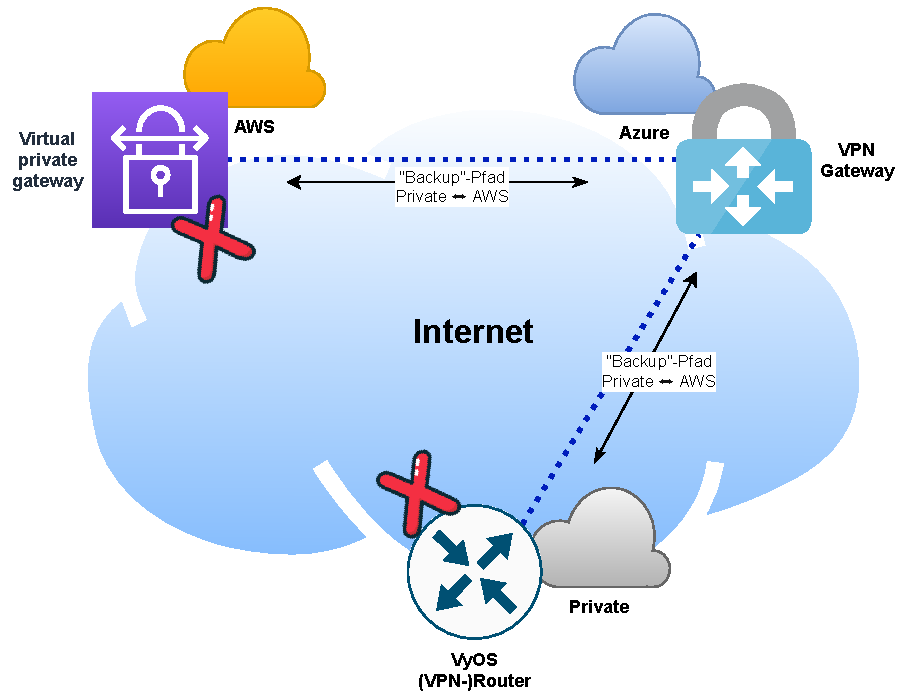
\includegraphics{Figures/Use-Case-1_Basis_Deployment_missing_link.pdf}
  \caption{Backbone mit einer fehlenden Verbindung zwischen Private Cloud und AWS.}
  \label{grafik:Use-Case-1_Basis_Deployment_missing_link}
\end{figure}\FloatBarrier

Man kann an Beispiel \ref{tf-base-deployment-ping-ok-missing-link} sehr gut erkennen, dass das BGP eine Konvergenzzeit erfordert, bis die Pakete über einen anderen Pfad laufen. \textit{ping} versendet in der Standardkonfiguration im Interval von einer Sekunde ICMP-Echo-Pakete. Daraus lässt sich schlussfolgern, dass die Verbindung in Beispiel \ref{tf-base-deployment-ping-ok-missing-link} etwa 44 Sekunden unterbrochen war.\\
Weiterhin hat sich die Round-Trip-Time von ~20 ms auf ~62 ms erhöht. Dies ist eine logische Konsequenz, da Pakete nun längere Wege (\textit{mehr Hops}) zurücklegen müssen. Alle Ping-Tests waren trotz Kappen einer Verbindung erfolgreich. Man muss dabei allerdings Paketverluste während der Konvergenzzeit hinnehmen.
%TC:ignore
\begin{listing}[h]
\begin{minted}[breaklines,frame=single]{bash}
root@www:~# ping 10.33.0.121
PING 10.33.0.121 (10.33.0.121) 56(84) bytes of data.
[...]
64 bytes from 10.33.0.121: icmp_seq=15 ttl=61 time=19.9 ms
64 bytes from 10.33.0.121: icmp_seq=16 ttl=61 time=24.3 ms
64 bytes from 10.33.0.121: icmp_seq=17 ttl=61 time=19.6 ms
64 bytes from 10.33.0.121: icmp_seq=18 ttl=61 time=19.7 ms 
--- Kappen einer Verbindung nach ICMP Sequenznummer 18 ---
--- Recovery zu ICMP Sequenznummer 62 via Backup-Pfad ----
64 bytes from 10.33.0.121: icmp_seq=62 ttl=61 time=67.4 ms
64 bytes from 10.33.0.121: icmp_seq=63 ttl=61 time=62.2 ms
64 bytes from 10.33.0.121: icmp_seq=64 ttl=61 time=62.5 ms
64 bytes from 10.33.0.121: icmp_seq=65 ttl=61 time=62.4 ms
[...]
\end{minted}
\caption{Ping-Tests zwischen verschiedenen Cloud-Plattformen mit Kappen einer Backbone-Verbindung.}
\label{tf-base-deployment-ping-ok-missing-link}
\end{listing}\FloatBarrier
%TC:endignore
Alle Evaluationskriterien (siehe \ref{eval-kriterien-uc1}) wurden somit erfüllt und der Use-Case konnte erfolgreich umgesetzt werden.